\documentclass{beamer}

\usetheme{Madrid}

\usepackage[colorlinks]{hyperref}
\usepackage{graphicx} % Include images in the presentation.
\usepackage{orcidlink} % Render oorcid ID properly. 
% \usepackage[style=verbose]{biblatex}
\usepackage[normalem]{ulem}

\title[\LaTeX] %optional
{\LaTeX is all you need}

\subtitle{This was made in \LaTeX in under 40 mins}

\author[jesse.wood@ecs.vuw.ac.nz] % (optional, for multiple authors)
{Jesse Wood\inst{1}\orcidlink{0000-0003-3756-2122} \and
    ChatGPT \inst{1}\orcidlink{0000-0002-6930-6863} \and
    Bing \inst{1}\orcidlink{0000-0003-4463-9538} \and
    LLaMA \inst{3}\orcidlink{0000-0002-4898-6724}
    Bard\inst{4}\orcidlink{0000-0002-4865-8026} \and
}

\institute[] % (optional)
{
    \inst{1}%
    School of Engineering and Computer Science | Te Kura Mātai Pūkaha, Pūrorohiko
    Victoria University of Wellington | Te Herenga Waka
  
    \inst{2}%
    Open AI | United States: San Francisco: Poineer building, 3180 18th St, San Francisco

    \inst{3}%
    Meta AI | Menlo Park, California, headquarters, London, United Kingdom, 

    \inst{4}%
    Google AI | 340 Main Street, Los Angeles, CA 90291, United States
}

\date{\today} % (optional)
{
    \snapper \bluecod \gurnard \tarakihi 
}

\logo{
\includegraphics[height=1cm]{assets/logos/vuw-logo.png}}

\newcommand{\snapper}{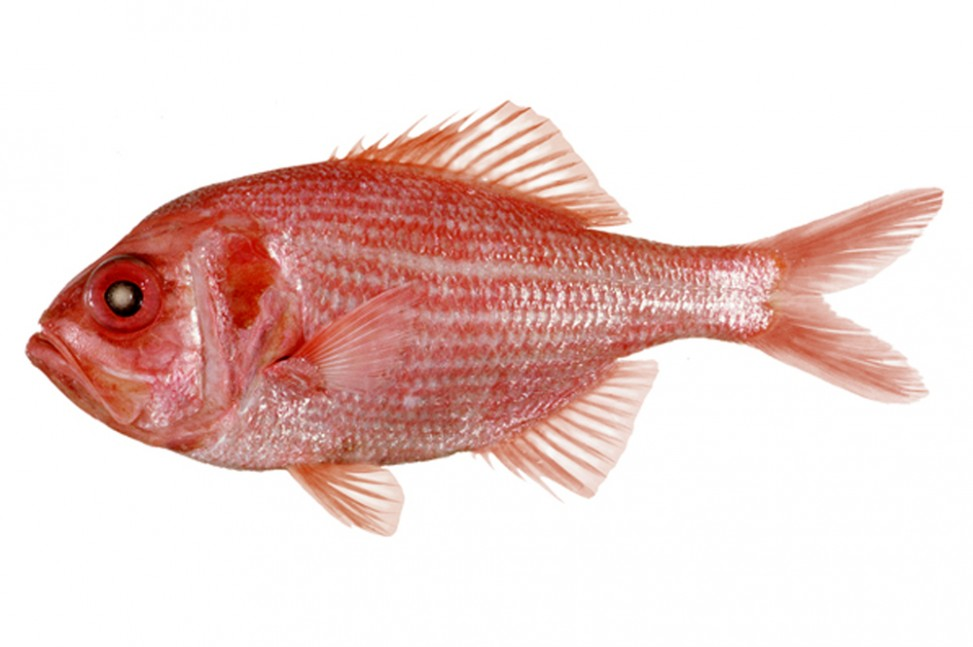
\includegraphics[height=0.5cm]{assets/fish/snapper.jpg}}
\newcommand{\bluecod}{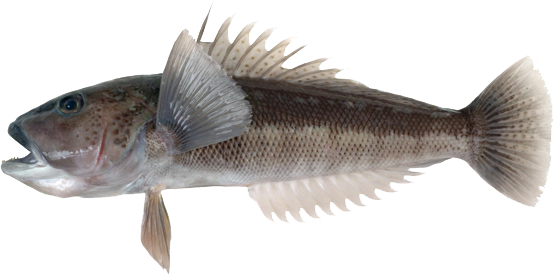
\includegraphics[height=0.5cm,width=0.8cm]{assets/fish/bluecod.png}}
\newcommand{\gurnard}{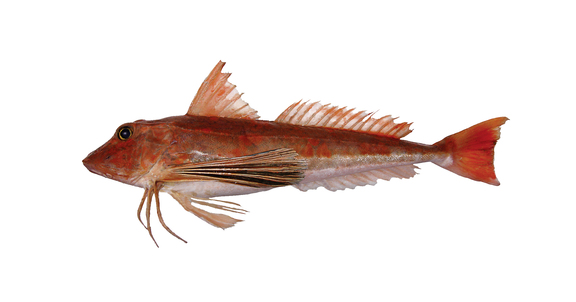
\includegraphics[height=0.5cm,width=1cm]{assets/fish/gurnard.jpg}}
\newcommand{\tarakihi}{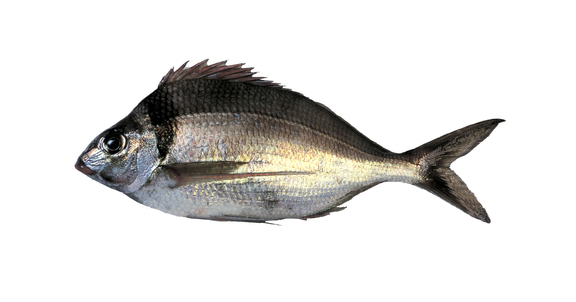
\includegraphics[height=0.5cm,width=1cm]{assets/fish/tarakihi.jpg}}
\newcommand{\parts}{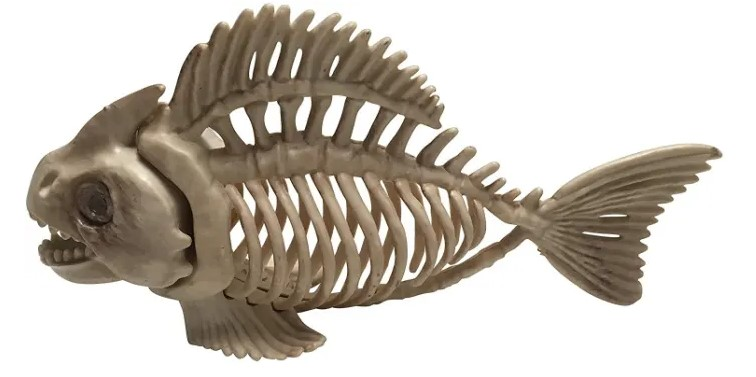
\includegraphics[height=0.5cm,width=1cm]{assets/fish/body-parts.jpg}}

\begin{document}
% Remove figure from captions (for some more room).
\setbeamertemplate{caption}{\raggedright\insertcaption\par}

\frame{\titlepage}

\begin{frame}{Tributes: Dominion Post}
\vspace{0.2cm}

Mum was a former journalist for what was then the "Evening Post", now the "Dominion Post". And had a tribute in the newspaper, both in print and on stuff.

\vspace{1cm}

\begin{figure}
    \centering
    
\includegraphics[height=0.3\textheight]{assets/qr/dominion_post_qr.png}
    \caption{Read Dominion Post Tribute}
    \label{fig:qr-code}
\end{figure}
\end{frame}

\begin{frame}{Tributes: Softball NZ}
\vspace{0.2cm}

Mum was a sports journalist who covered Softball in New Zealand. She then went on to work for Softball New Zealand as an Office Director.

\vspace{1cm}

\begin{figure}
    \centering
    
\includegraphics[height=0.3\textheight]{assets/qr/softball_nz_qr.png}
    \caption{Read Softball NZ Tribute}
    \label{fig:qr-code}
\end{figure}
\end{frame}

\begin{frame}{Funeral: St. Hildas Church, Island Bay}
    \centering
    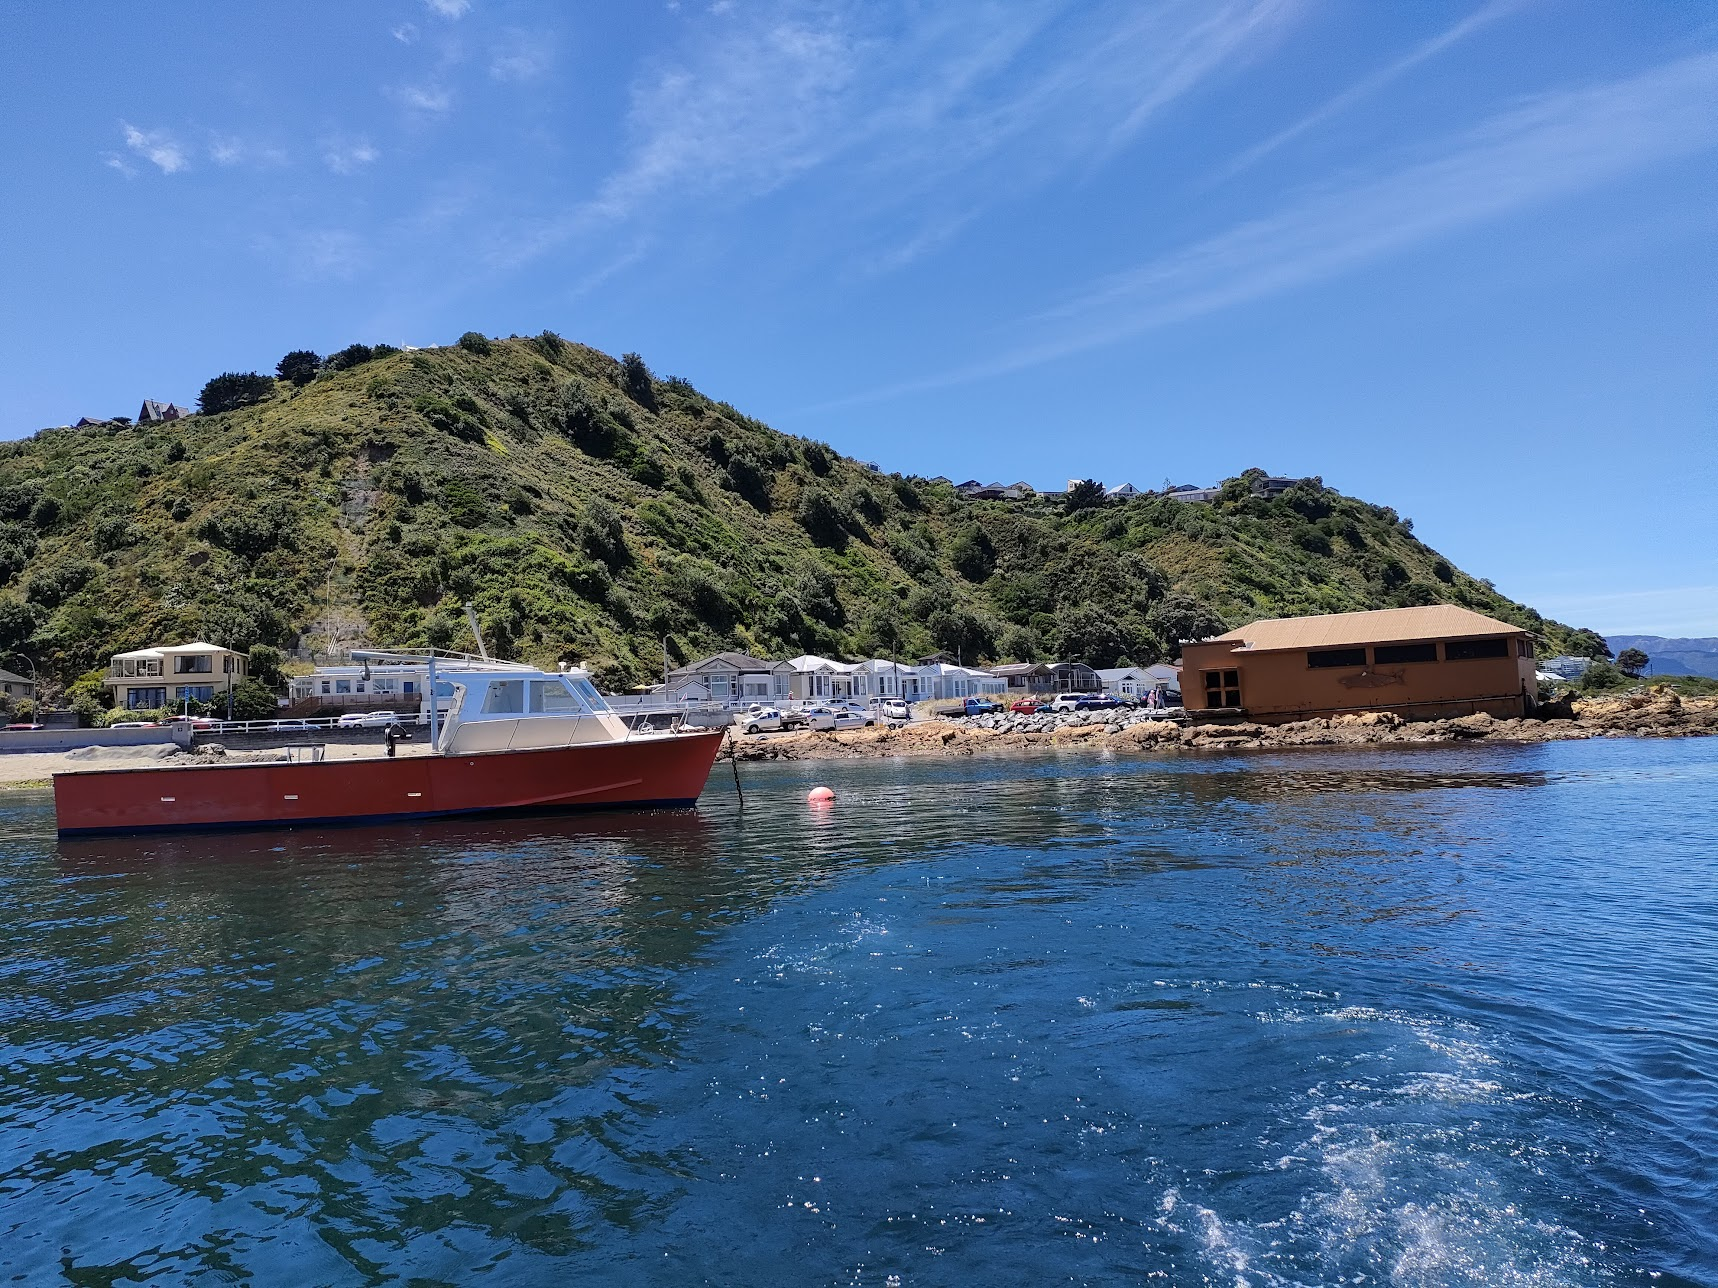
\includegraphics[width=\linewidth]{assets/island-bay.jpg}
\end{frame}

\begin{frame}{Funeral: Live performance}

\begin{figure}
    \centering
    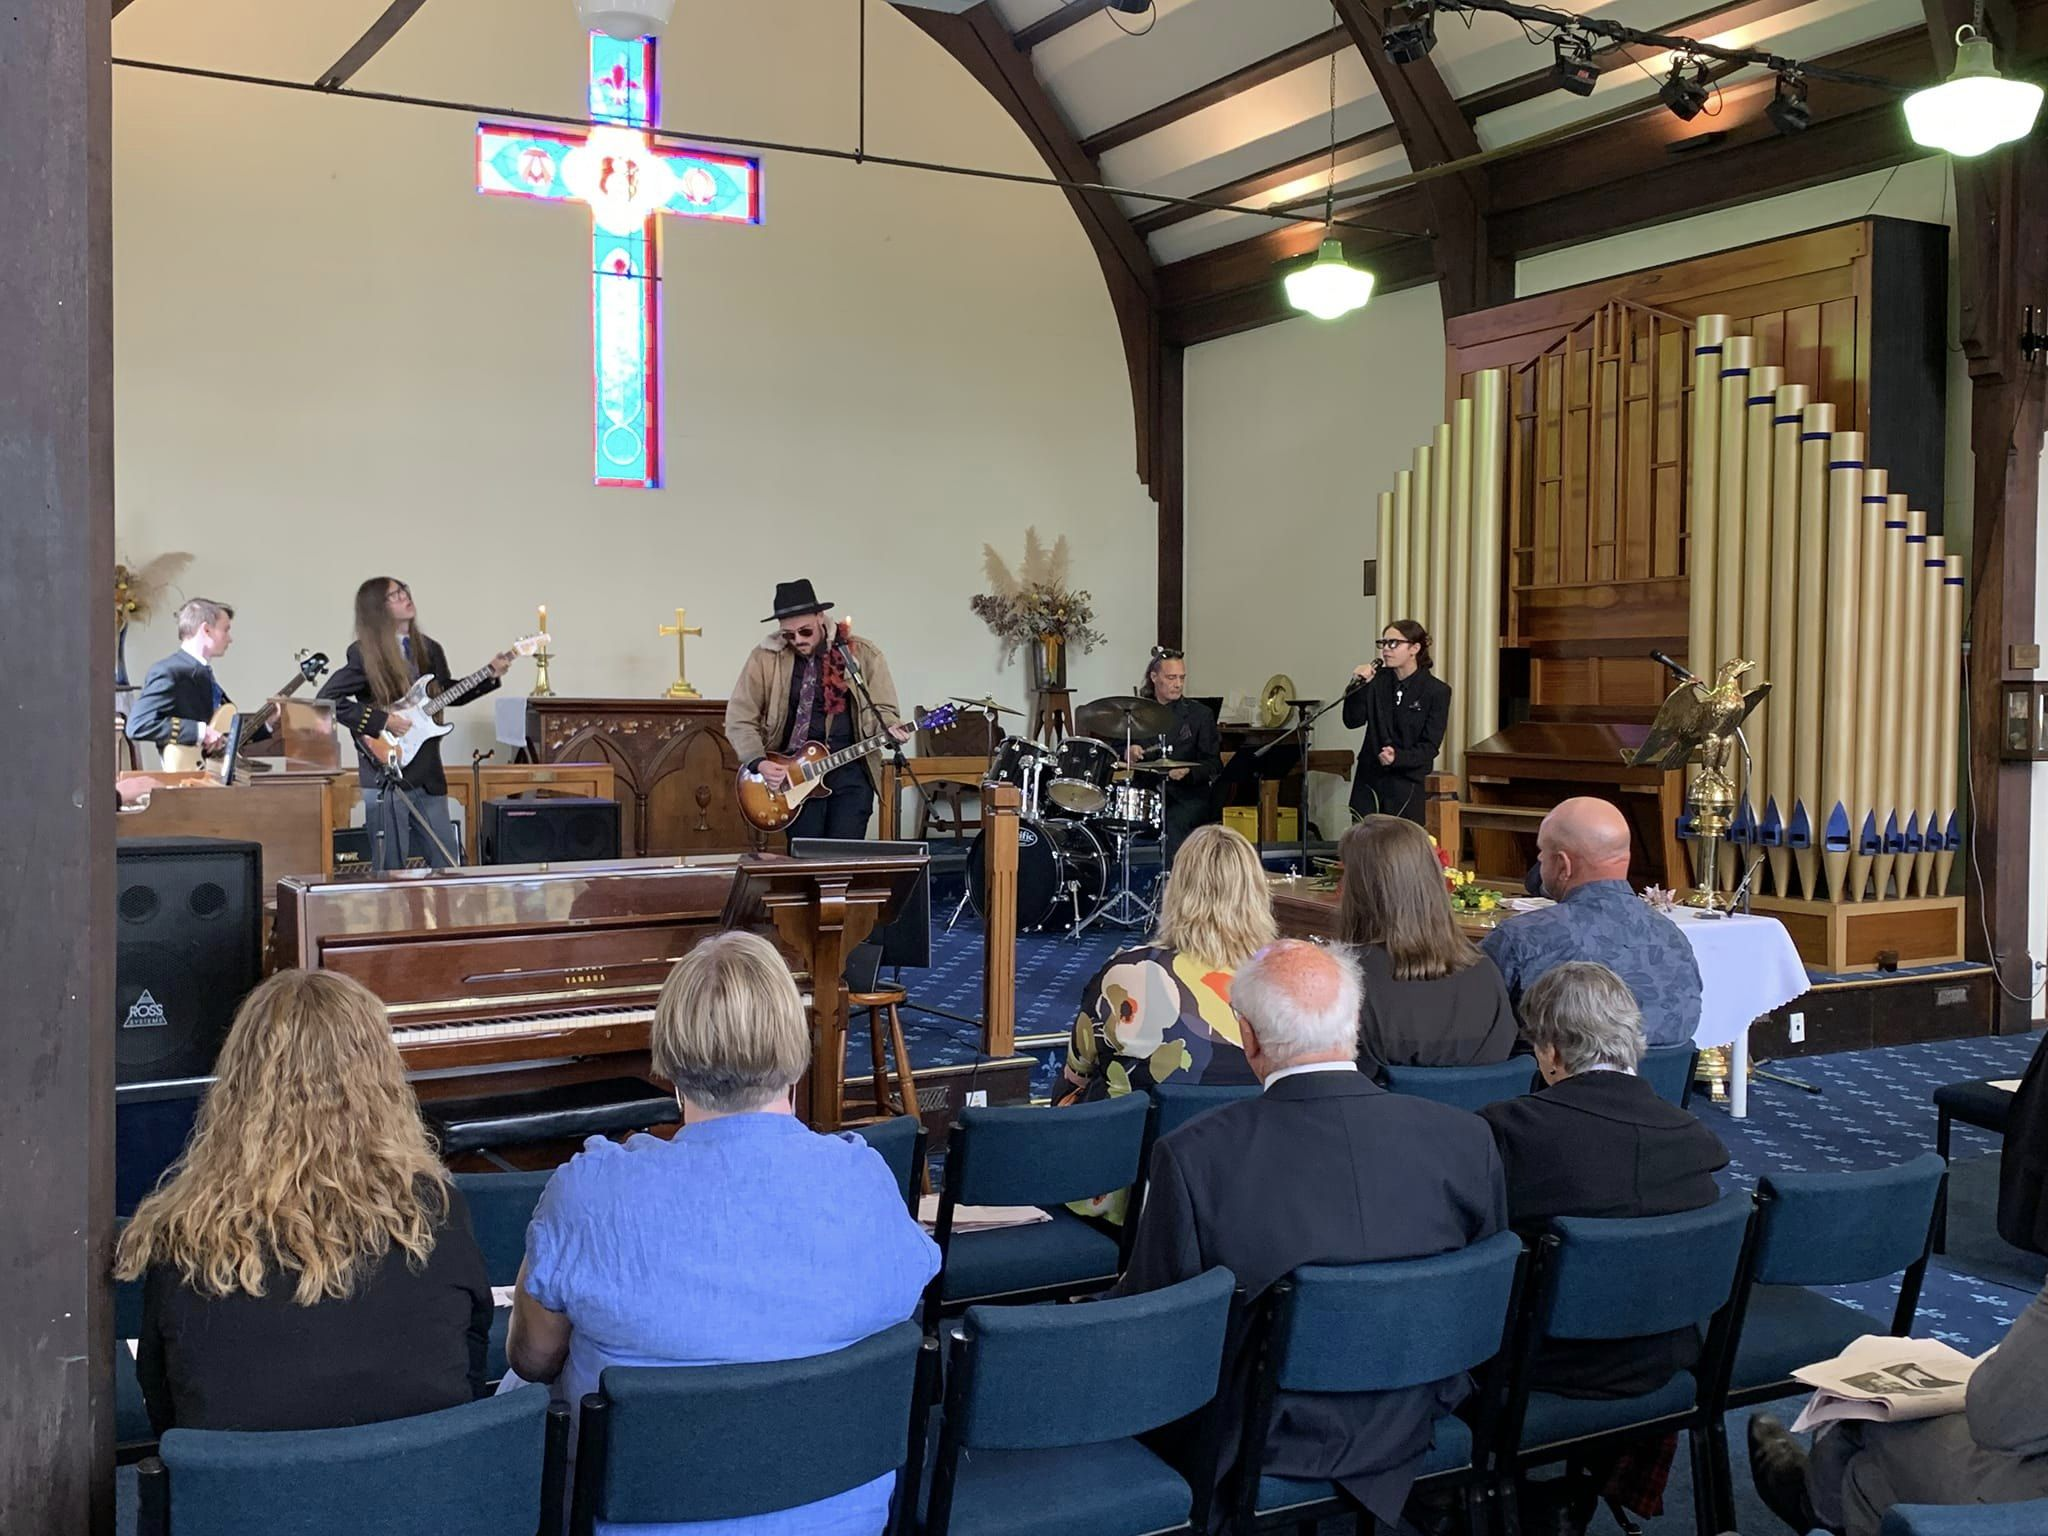
\includegraphics[width=\linewidth]{assets/wont_get_fooled_again.jpg}
    \caption{Service sheet was made in \LaTeX!}
    \label{fig:qr-code}
\end{figure}
\end{frame}

\begin{frame}{Service Sheet (well not quite!)}

\begin{figure}
    \centering
    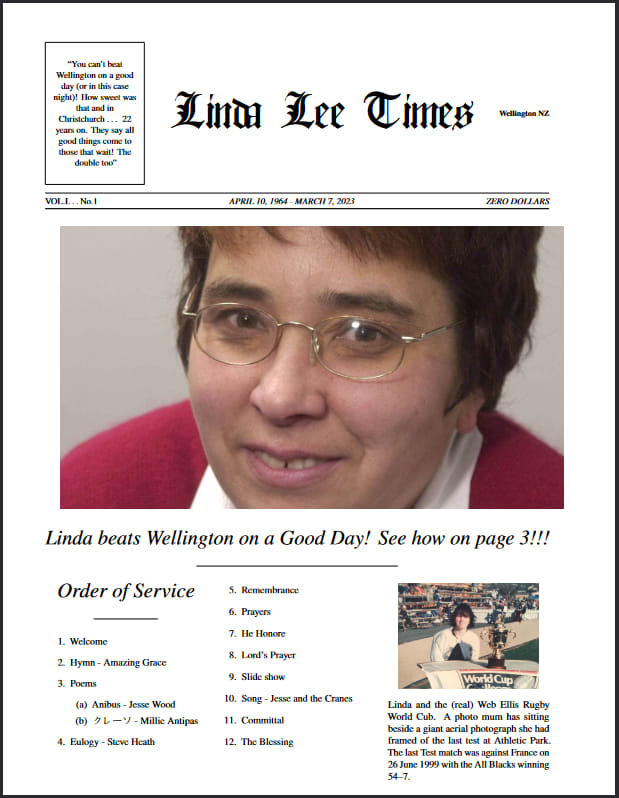
\includegraphics[height=0.7\textheight]{assets/Linda_Lee_Times.jpg}
    \caption{made in \LaTeX!}
    \label{fig:qr-code}
\end{figure}
\end{frame}

\begin{frame}{Thank you for listening!}
\vspace{0.2cm}

In lieu of donations,

\sout{
    wire ethereum directly to my cold wallet here: 
    \\ 
    \$ETH $\to$ 0x045BA9c0c69AF53B2Fca0e1A3769E44D9a328696
}

\vspace{1cm}

\begin{figure}
    \centering
    
\includegraphics[height=0.3\textheight]{assets/qr/wellington_free_qr.png}
    \caption{Donate to Wellington Free Ambulance (hint: ask Jordan)}
    \label{fig:qr-code}
\end{figure}
\end{frame}

\begin{frame}{Funeral: Live performance (without noise control complaints}

\begin{figure}
    \centering
    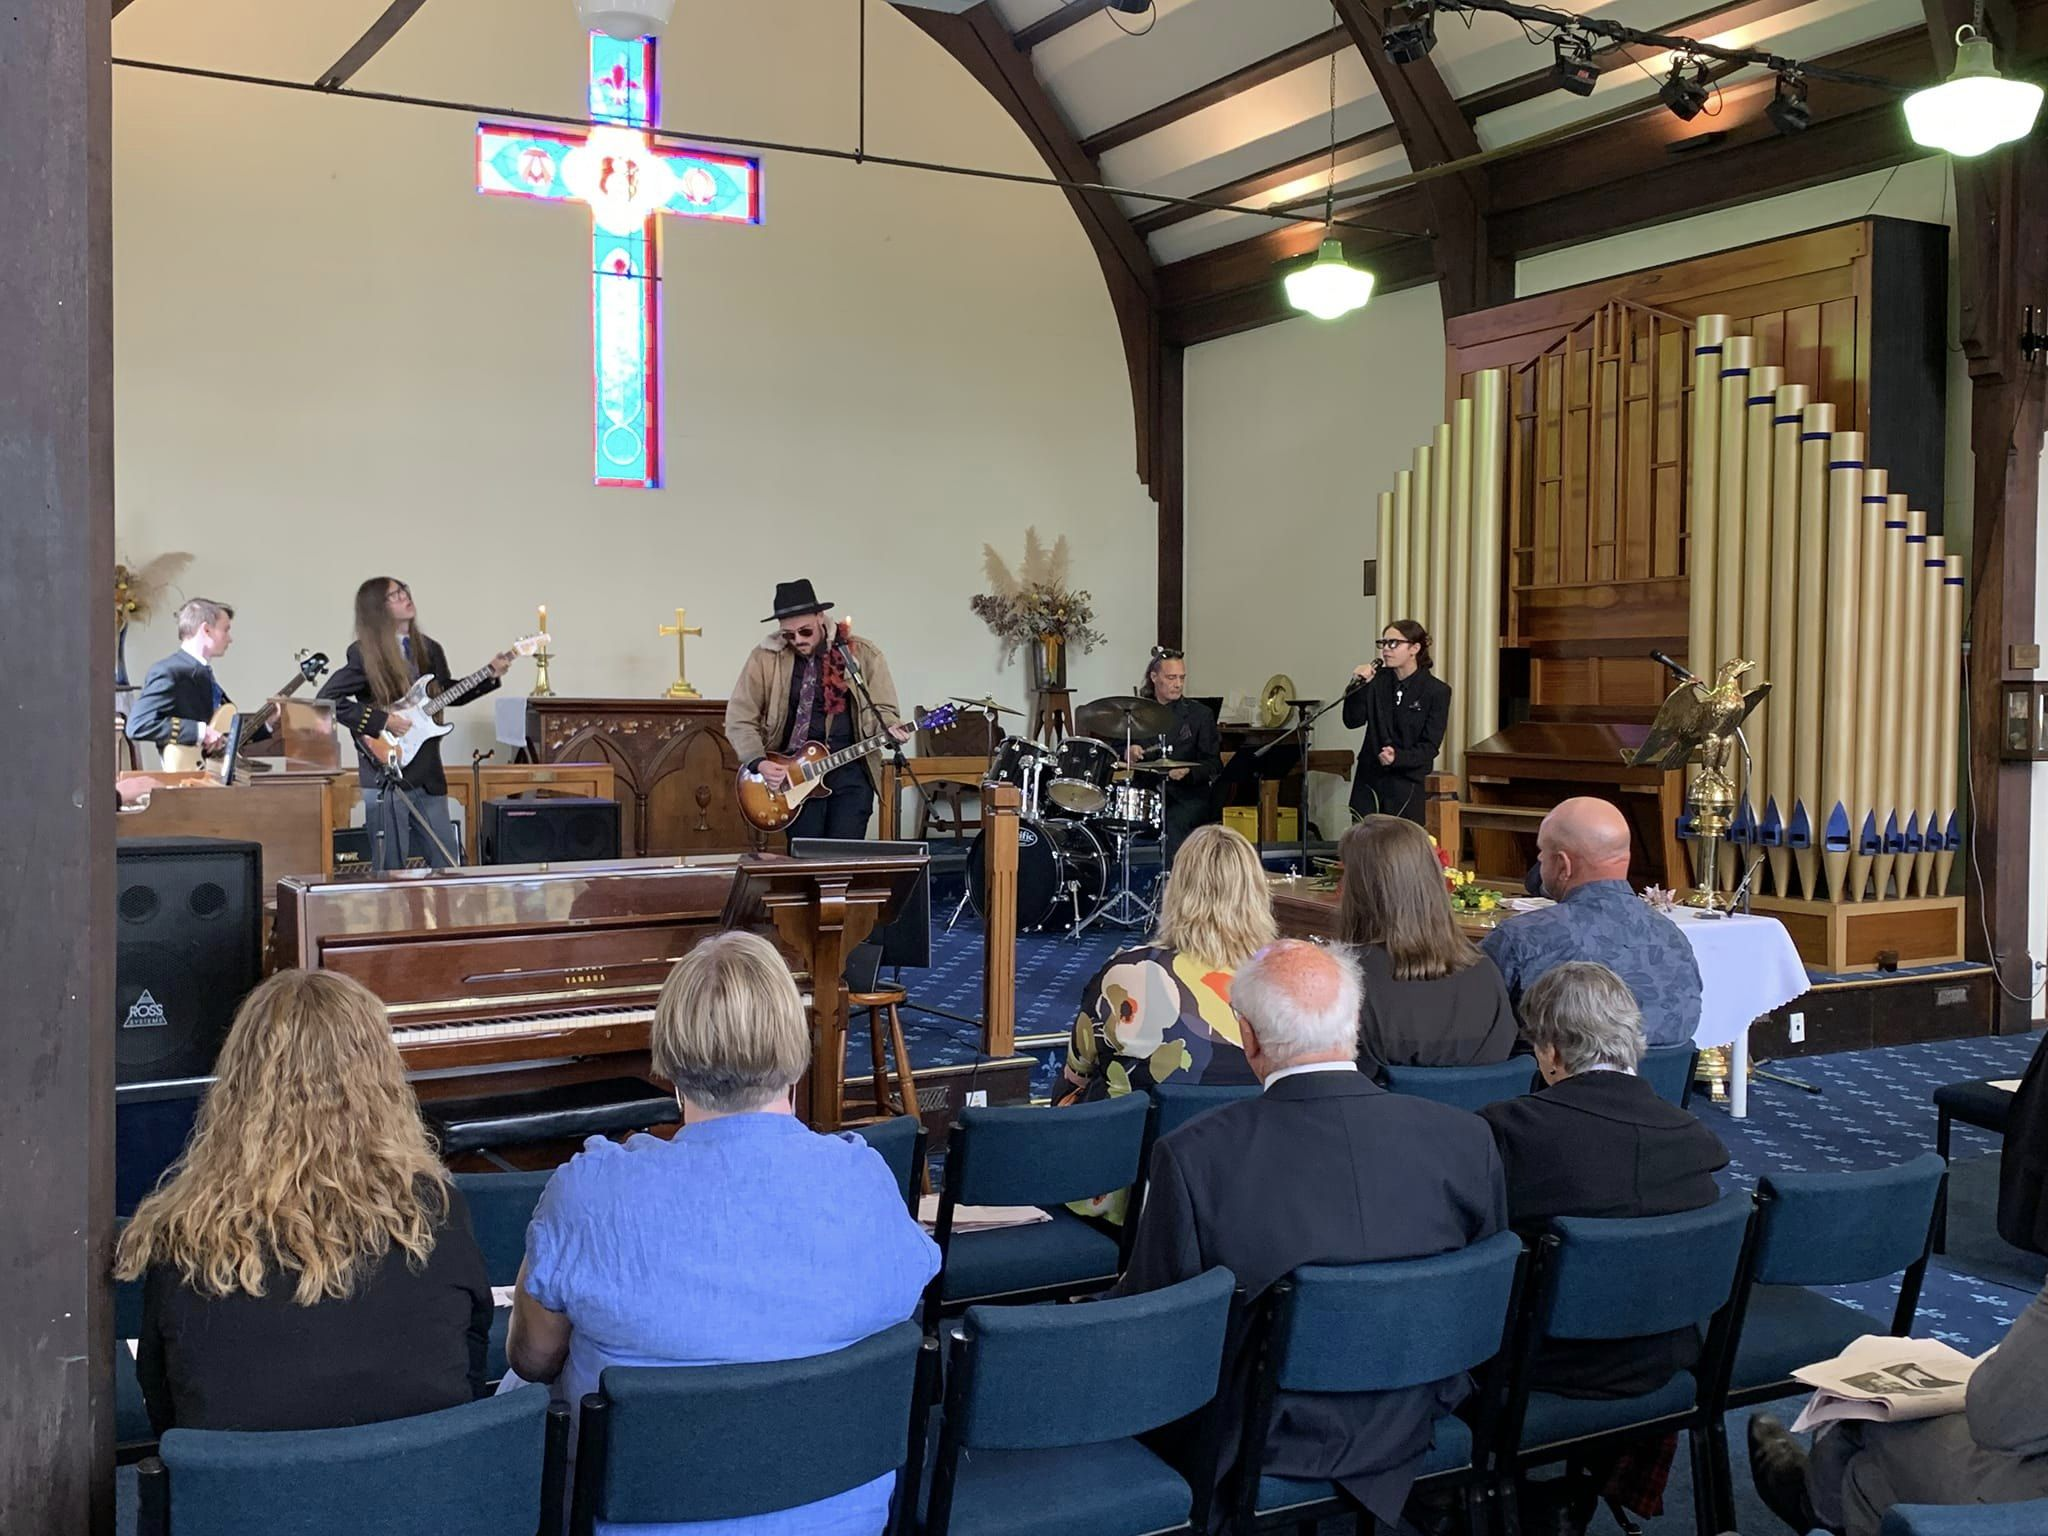
\includegraphics[width=\linewidth]{assets/wont_get_fooled_again.jpg}
    \caption{Service sheet was made in \LaTeX!}
    \label{fig:qr-code}
\end{figure}
\end{frame}

% Make the bibliography an ordered list (source: https://bit.ly/3MGKmGN)
\setbeamertemplate{bibliography item}{\insertbiblabel}

\bibliographystyle{IEEEtran}
\bibliography{refs}

\end{document}